\documentclass{article}
\usepackage{graphicx}
\usepackage[utf8]{inputenc}
\usepackage{amsmath, amssymb, latexsym}

\usepackage{pgfplots}
\usepackage{algorithm}
\usepackage[noend]{algpseudocode}
\usepackage{tikz}
\usepackage{nicefrac}
\pgfplotsset{every axis legend/.append style={
at={(0,0)},
anchor=north east}}
\usetikzlibrary{shapes,positioning,intersections,quotes}
\usetikzlibrary{arrows.meta,
                bending,
                intersections,
                quotes,
                shapes.geometric}
                
\definecolor{darkgreen}{rgb}{0.0, 0.6, 0.0}
\definecolor{darkred}{rgb}{0.7, 0.0, 0.0}
\makeatletter
\def\BState{\State\hskip-\ALG@thistlm}
\makeatother
\title{Week 6}
\begin{document}
  \pagenumbering{gobble}
  \maketitle
  \newpage
  \pagenumbering{arabic}

\section*{Classification}
\begin{itemize}
\item Y can only have discrete values.
\item For example: 0 = negative class (absence of something) and 1 = positive class (presence of something).
\item Email $->$ spam/not spam?
\item Online transactions $->$ fraudulent?
\item Tumor $->$ Malignant/benign?
\end{itemize}

Let's go back to the cancer example from the Week 1 and try to apply linear regression:

~\\
\begin{tikzpicture}
    \begin{axis}[
        axis x line=middle,
        axis y line=middle,
        width=12cm, height=5cm,     % size of the image
        grid = none,
        grid style={dashed, gray!0},
        %xmode=log,log basis x=10,
        %ymode=log,log basis y=10,
        xmin=0,     % start the diagram at this x-coordinate
        xmax= 1,    % end   the diagram at this x-coordinate
        ymin=-0.1,     % start the diagram at this y-coordinate
        ymax= 2.5,   % end   the diagram at this y-coordinate
        %/pgfplots/xtick={0,1,...,60}, % make steps of length 5
        %extra x ticks={23},
        extra y ticks={0, 1},
        axis background/.style={fill=white},
        ylabel=Maligant?,
        xlabel=Tumor size,
        xticklabels={,,},
        yticklabels={,,},
        tick align=outside,
        tension=0.08]
      % plot the stirling-formulae
       \fill[blue] (5, 5) circle (5pt);
       \fill[blue] (20, 5) circle (5pt);
       \fill[blue] (30, 5) circle (5pt);
       \fill[blue] (50, 5) circle (5pt);
       \fill[blue] (60, 5) circle (5pt);
       \fill[red] (50, 20) circle (5pt);
       \fill[red] (45, 20) circle (5pt);
       \fill[red] (65, 20) circle (5pt);
       \fill[red] (75, 20) circle (5pt);
       \fill[red] (89, 20) circle (5pt);
      \addplot[domain=0:10, gray, ultra thick,samples=500] {2.5*x - 0.3};

    \end{axis}
    	\node[above,font=\large\bfseries] at (current bounding box.north) {Define breast cancer as malignant or benign based on tumour size
};
\end{tikzpicture}

~\\
We see that it wasn't the best idea. Of course, we could attempt another approach to find a straight line that would better separate the points, but a straight line isn't our sole choice. There are more appropriate functions for that job.

\section*{Hypothesis representation}
\begin{itemize}
\item We want our classifier to output values between 0 and 1.
\item For classification hypothesis representation we have: $h_{\theta}(x) = g((\theta^Tx))$.
\item $g(z)$ is called the sigmoid function, or the logistic function.
$$g(z) = \frac{1}{1 + e^{-z}}$$
\item If we combine these equations we can write out the hypothesis as:
\end{itemize}

$$h_{\theta}(x) = \frac{1}{1+e^{-\theta Tx}}$$

~\\
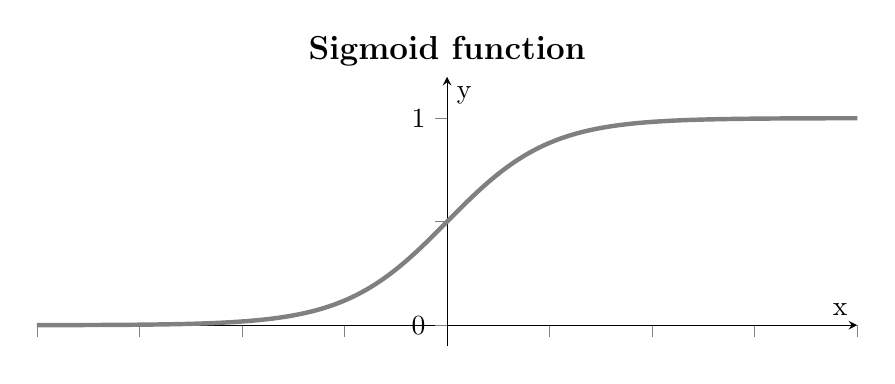
\begin{tikzpicture}
    \begin{axis}[
        axis x line=middle,
        axis y line=middle,
        width=12cm, height=5cm,     % size of the image
        grid = none,
        grid style={dashed, gray!0},
        %xmode=log,log basis x=10,
        %ymode=log,log basis y=10,
        xmin= -8,     % start the diagram at this x-coordinate
        xmax= 8,    % end   the diagram at this x-coordinate
        ymin=-0.1,     % start the diagram at this y-coordinate
        ymax= 1.2,   % end   the diagram at this y-coordinate
        %/pgfplots/xtick={0,1,...,60}, % make steps of length 5
        %extra x ticks={23},
        extra y ticks={0, 1},
        axis background/.style={fill=white},
        ylabel=y,
        xlabel=x,
        xticklabels={,,},
        yticklabels={,,},
        tick align=outside,
        tension=0.08]
      % plot the stirling-formulae
      \addplot[domain=-8:8, gray, ultra thick,samples=500] {1/(1+exp(-x)};

    \end{axis}
    	\node[above,font=\large\bfseries] at (current bounding box.north) {Sigmoid function
};
\end{tikzpicture}

~\\
When our hypothesis $(h_{\theta}(x))$ outputs a number, we treat that value as the estimated probability that $y=1$ on input $x$.

$$h_{\theta}(x) = P(y=1|x\ ;\ \theta)$$

~\\
Example:\\

$h_{\theta}(x) = 0.7$ and

 \begin{align*}
    X &= \begin{bmatrix}
           1 \\
           tumourSize
         \end{bmatrix}
  \end{align*}

~\\
Informs a patient that a tumor has a $70\%$ likelihood of being malignant.

\section*{Decision boundary}

One way of using the sigmoid function is:

\begin{itemize}
\item When the probability of y being 1 is greater than 0.5 then we can predict y = 1.
\item Else we predict y = 0.
\end{itemize}

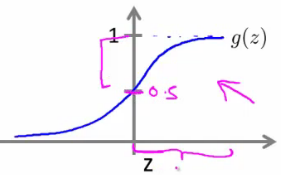
\includegraphics[width=0.5\textwidth]{resources/decision_boundary}

\begin{itemize}
\item The hypothesis predicts $y = 1$ when $\theta^T  x >= 0$.
\item When $\theta^T x <= 0$ then the hypothesis predicts y = 0.
\end{itemize}

~\\
Example

$$h_{\theta}(x) = g(\theta_0 + \theta_1x_1 + \theta_2x_2)$$

\begin{align*}
 \theta &= \begin{bmatrix}
    -3 \\
    1 \\
    1
 \end{bmatrix}
\end{align*}

~\\
We predict $y = 1$ if:

$$-3x_0 + 1x_1 + 1x_2 \geq 0$$
$$-3 + x_1 + x_2 \geq 0$$

~\\
As a result, the straight line equation is as follows:
$$x_2 = -x_1 + 3$$

~\\\\
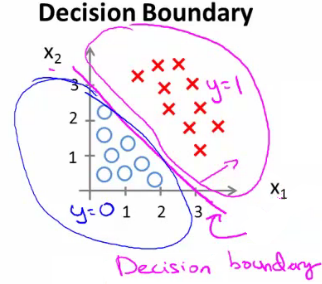
\includegraphics[width=0.5\textwidth]{resources/linear_decision_boundary}

\begin{itemize}
\item Blue = false
\item Magenta = true
\item Line = decision boundary
\end{itemize}

\section*{Non-linear decision boundaries}

Get logistic regression to fit a complex non-linear data set.

~\\
Example
$$h_{\theta}(x) = g(\theta_0 + \theta_1x_1 + \theta_3x_1^2 + \theta_4x_2^2)$$

\begin{align*}
 \theta &= \begin{bmatrix}
    -1 \\
    0 \\
    0 \\
    1 \\
    1
 \end{bmatrix}
\end{align*}

~\\
We predict $y = 1$ if:

$$-1 + x_1^2 + x_2^2 \geq 0$$
$$x_1^2 + x_2^2 \geq 1$$

~\\
As a result, the circle equation is as follows:
$$x_1^2 + x_2^2 = 1$$

~\\
This gives us a circle with a radius of 1 around 0.

~\\\\
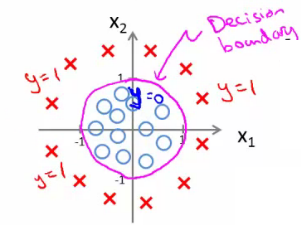
\includegraphics[width=0.5\textwidth]{resources/non_linear_decision_boundary}

\section*{Cost function for logistic regression}

\begin{itemize}
\item Fit $\theta$ parameters/
\item Define the optimization object for the cost function we use the fit the parameters.
\end{itemize}

~\\
Training set of m training examples:
$$\{(x^{(1)}, y^{(1)}), (x^{(1)}, y^{(1)}), ..., (x^{(m)}, y^{(m)})\}$$

\begin{align*}
 x &= \begin{bmatrix}
    x_0 \\
    x_1 \\
    ... \\
    x_n 
 \end{bmatrix}
\end{align*}

$$x_0 =1,\quad y \in \{0,1\}$$

~\\
Linear regression uses the following function to determine $\theta$:

$$J(\theta) = \frac{1}{2m} \sum_{m}^{i=1}(h_{\theta}(x^{(i)}) - y^{(i)})^2$$

~\\
We define "cost()" as:

$$cost(h_{\theta}(x^{(i)}), y^{(i)}) = \frac{1}{2} (h_{\theta}(x^{(i)}) - y^{(i)})^2$$

~\\
We can now redefine $J(\theta)$ as:

$$J(\theta) = \frac{1}{2} \sum_{m}^{i=1}cost(h_{\theta}(x^{(i)}), y^{(i)})$$

\begin{itemize}
\item This is the cost you want the learning algorithm to pay if the outcome is $h_{\theta}(x)$ but the actual outcome is y.
\item This function is a non-convex function for parameter optimization when used for logistic regression.
\item If you take $h_{\theta}(x)$ and plug it into the Cost() function, and them plug the Cost() function into $J(\theta)$ and plot $J(\theta)$ we find many local optimum.
\end{itemize}

    \[ cost(h_{\theta}(x), y) = \begin{cases} 
          -log(h_{\theta}(x)) & if\ y=1 \\
          -log(1 - h_{\theta}(x)) & if\ y=0
       \end{cases}
    \]

\section*{Multiclass classification problems}
Getting logistic regression for multiclass classification using one vs. all.

~\\
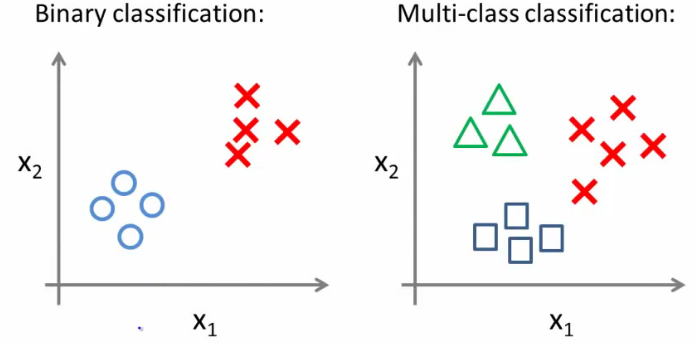
\includegraphics[width=0.8\textwidth]{resources/multiclass_classification}

~\\
Split the training set into three separate binary classification problems.
\begin{itemize}
\item Triangle (1) vs crosses and squares (0) $h_{\theta}^{(1)}(x)$.
\item Crosses (1) vs triangle and square (0) $h_{\theta}^{(2)}(x)$.
\item Square (1) vs crosses and square (0) $h_{\theta}^{(3)}(x)$. 
\end{itemize}

~\\
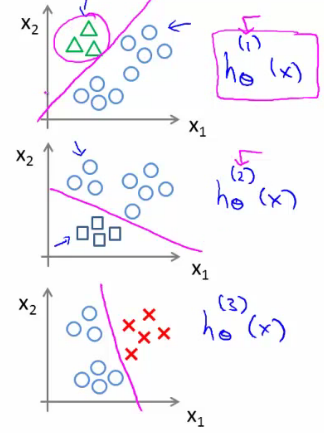
\includegraphics[width=0.5\textwidth]{resources/one_vs_all}


\end{document}